\section[Binomial Ancova]{Ancova with a Binary Response Variable }

\begin{frame}[fragile]\frametitle{Parasite Infection Example}
\begin{itemize}
\item the binary response variable is parasite infection (infected or not) 
\item the explanatory variables are weight and age (continuous) 
\item and sex (categorical)
\item we want to investigate if there is a different effect of age for each of the sexes on the outcome variable
\end{itemize}
\begin{exampleblock}{Input/Output}\footnotesize
\begin{verbatim}
> load("infection.rdata")
> summary(infection)
         infected        age             sex     
 infected    :338   Min.   :  2.00   female:243  
 not infected:162   1st Qu.: 46.00   male  :257  
                    Median : 84.50               
                    Mean   : 93.69               
                    3rd Qu.:139.25               
                    Max.   :200.00               
\end{verbatim}
\end{exampleblock}

\end{frame}


\begin{frame}[fragile]\frametitle{Parasite Infection Example}\footnotesize
  \begin{exampleblock}{Input/Output}\scriptsize
\begin{verbatim}
> m.inf <- glm(infected~age*sex,family=binomial,
+                               data=infection)
> summary(m.inf)
Call:
glm(formula = infected ~ age * sex, family = binomial, 
                                     data = infection)
Deviance Residuals: 
    Min       1Q   Median       3Q      Max  
-2.0411  -0.7307  -0.4363   0.6632   2.3215  
Coefficients:
             Estimate Std. Error z value Pr(>|z|)    
(Intercept) -3.000513   0.413639  -7.254 4.05e-13 ***
age          0.015657   0.003176   4.929 8.25e-07 ***
sex          0.116664   0.553956   0.211   0.8332    
age:sex      0.011050   0.004612   2.396   0.0166 *  

(Dispersion parameter for binomial family taken to be 1)
    Null deviance: 629.85  on 499  degrees of freedom
Residual deviance: 477.61  on 496  degrees of freedom
AIC: 485.61
\end{verbatim}
  \end{exampleblock}

\end{frame}

\begin{frame}[fragile]\frametitle{Parasite Infection Example}
\begin{itemize}
\item so for male at a age of 0 there is a probability of
    \begin{exampleblock}{Input/Output}
\begin{verbatim}
> invlogit(coef(m.inf)[1])
(Intercept) 
 0.04740269 
\end{verbatim}
    \end{exampleblock}
  \item for females the probability at age 0 is
    \begin{exampleblock}{Input/Output}
\begin{verbatim}
> invlogit(coef(m.inf)[1]+coef(m.inf)[3])
(Intercept) 
 0.05295775 
\end{verbatim}
  \end{exampleblock}
\end{itemize}
\end{frame}


\begin{frame}[fragile]\frametitle{Compare Slopes}
\begin{itemize}
\item so what about the slope?
\item for males the underlying model is the following
$$\mbox{Pr(infection)}=\mbox{logit}^{-1}(-3.000513 + 0.015657 \cdot \mbox{age}) $$
\item for females the slope is almost twice as high
  $$\mbox{Pr(infection)}=\mbox{logit}^{-1}(-2.883849 + 0.02670685  \cdot \mbox{age}) $$
\end{itemize}
\end{frame}


\begin{frame}[fragile]\frametitle{Compare Slopes}
\begin{itemize}
\item looking at the odds ratios (which seem to be rather small)
\item for males and females:
  \begin{exampleblock}{Input/Output}\small
\begin{verbatim}
> exp(coef(m.inf)[2]) ## males
    age 
1.01578 
> exp(coef(m.inf)[2] + coef(m.inf)[4]) ## females
     age  
1.027067 
\end{verbatim}
  \end{exampleblock}
\item these are the odds ratios for +1 time unit
\end{itemize}
\end{frame}

\begin{frame}[fragile]\frametitle{Compare Slopes}
  \begin{itemize}
  \item if time unit is days you get the odds ratio for +1 month   by
  \begin{exampleblock}{Input/Output}\small
\begin{verbatim}
> exp(30 * coef(m.inf)[2])
     age 
1.599512 
> exp(30 * (coef(m.inf)[2] + coef(m.inf)[4]))
     age 
2.228225 
\end{verbatim}
  \end{exampleblock}
\item so keep in mind the scale you are measuring on
\end{itemize}
\end{frame}

  \begin{frame}[fragile]\frametitle{Compare Slopes}
\begin{itemize}
\item we can also compare them by looking at the age where the probability to be infected is 50\%
\item this is the case when $$-3.000513 + 0.015657 \cdot \mbox{age}=0$$  respectively $$-2.883849 + 0.02670685  \cdot \mbox{age}=0$$ you can do it by hand or use R
\end{itemize}
\end{frame}

\begin{frame}[fragile]\frametitle{Compare Slopes}
\begin{itemize}
\item \texttt{solve()} solves systems of linear equations in the form A*x=b, where A is the matrix of coefficients and b are the (negative) intercepts, here we have the special case with just one equation
  \begin{exampleblock}{Input/Output}\small
\begin{verbatim}
> ## male
> solve(0.015657,3.000513)
[1] 191.6404
> ## female
> solve(0.02670685,2.883849)
[1] 107.9816
\end{verbatim}
  \end{exampleblock}

\end{itemize}
\end{frame}

\begin{frame}[fragile]\frametitle{Compare Effects}
\begin{itemize}
\item you can also use the \texttt{allEffects()} function (part of the \texttt{effects} package), which give you the probabilities for being infected on several ages for both sexes
  \begin{exampleblock}{Input/Output}\scriptsize
\begin{verbatim}
> allEffects(m.inf)
 model: infected ~ age * sex

 age*sex effect
     sex
age            0          1
  2   0.04883687 0.05570148
  24  0.06756215 0.09596497
  46  0.09276694 0.16038932
  68  0.12610300 0.25582483
  90  0.16918450 0.38219715
  112 0.22322468 0.52680374
  134 0.28853152 0.66704908
  156 0.36399154 0.78286130
  178 0.44679328 0.86645480
  200 0.53265591 0.92110968
\end{verbatim}
  \end{exampleblock}

\end{itemize}
\end{frame}


\begin{frame}[fragile]\frametitle{Compare Effects}
\begin{itemize}
\item choose values of age
  \begin{exampleblock}{Input/Output}\footnotesize
\begin{verbatim}
> allEffects(m.inf,
+            xlevels = list(age = seq(0,200,by = 50)))
 model: infected ~ age * sex

 age*sex effect
     sex
age       female       male
  0   0.04740269 0.05295775
  50  0.09817379 0.17530204
  100 0.19234385 0.44690980
  150 0.34253427 0.75439251
  200 0.53265591 0.92110968
\end{verbatim}
  \end{exampleblock}

\end{itemize}
\end{frame}

\begin{frame}[fragile]\frametitle{Parasite Infection graph}
\begin{center}
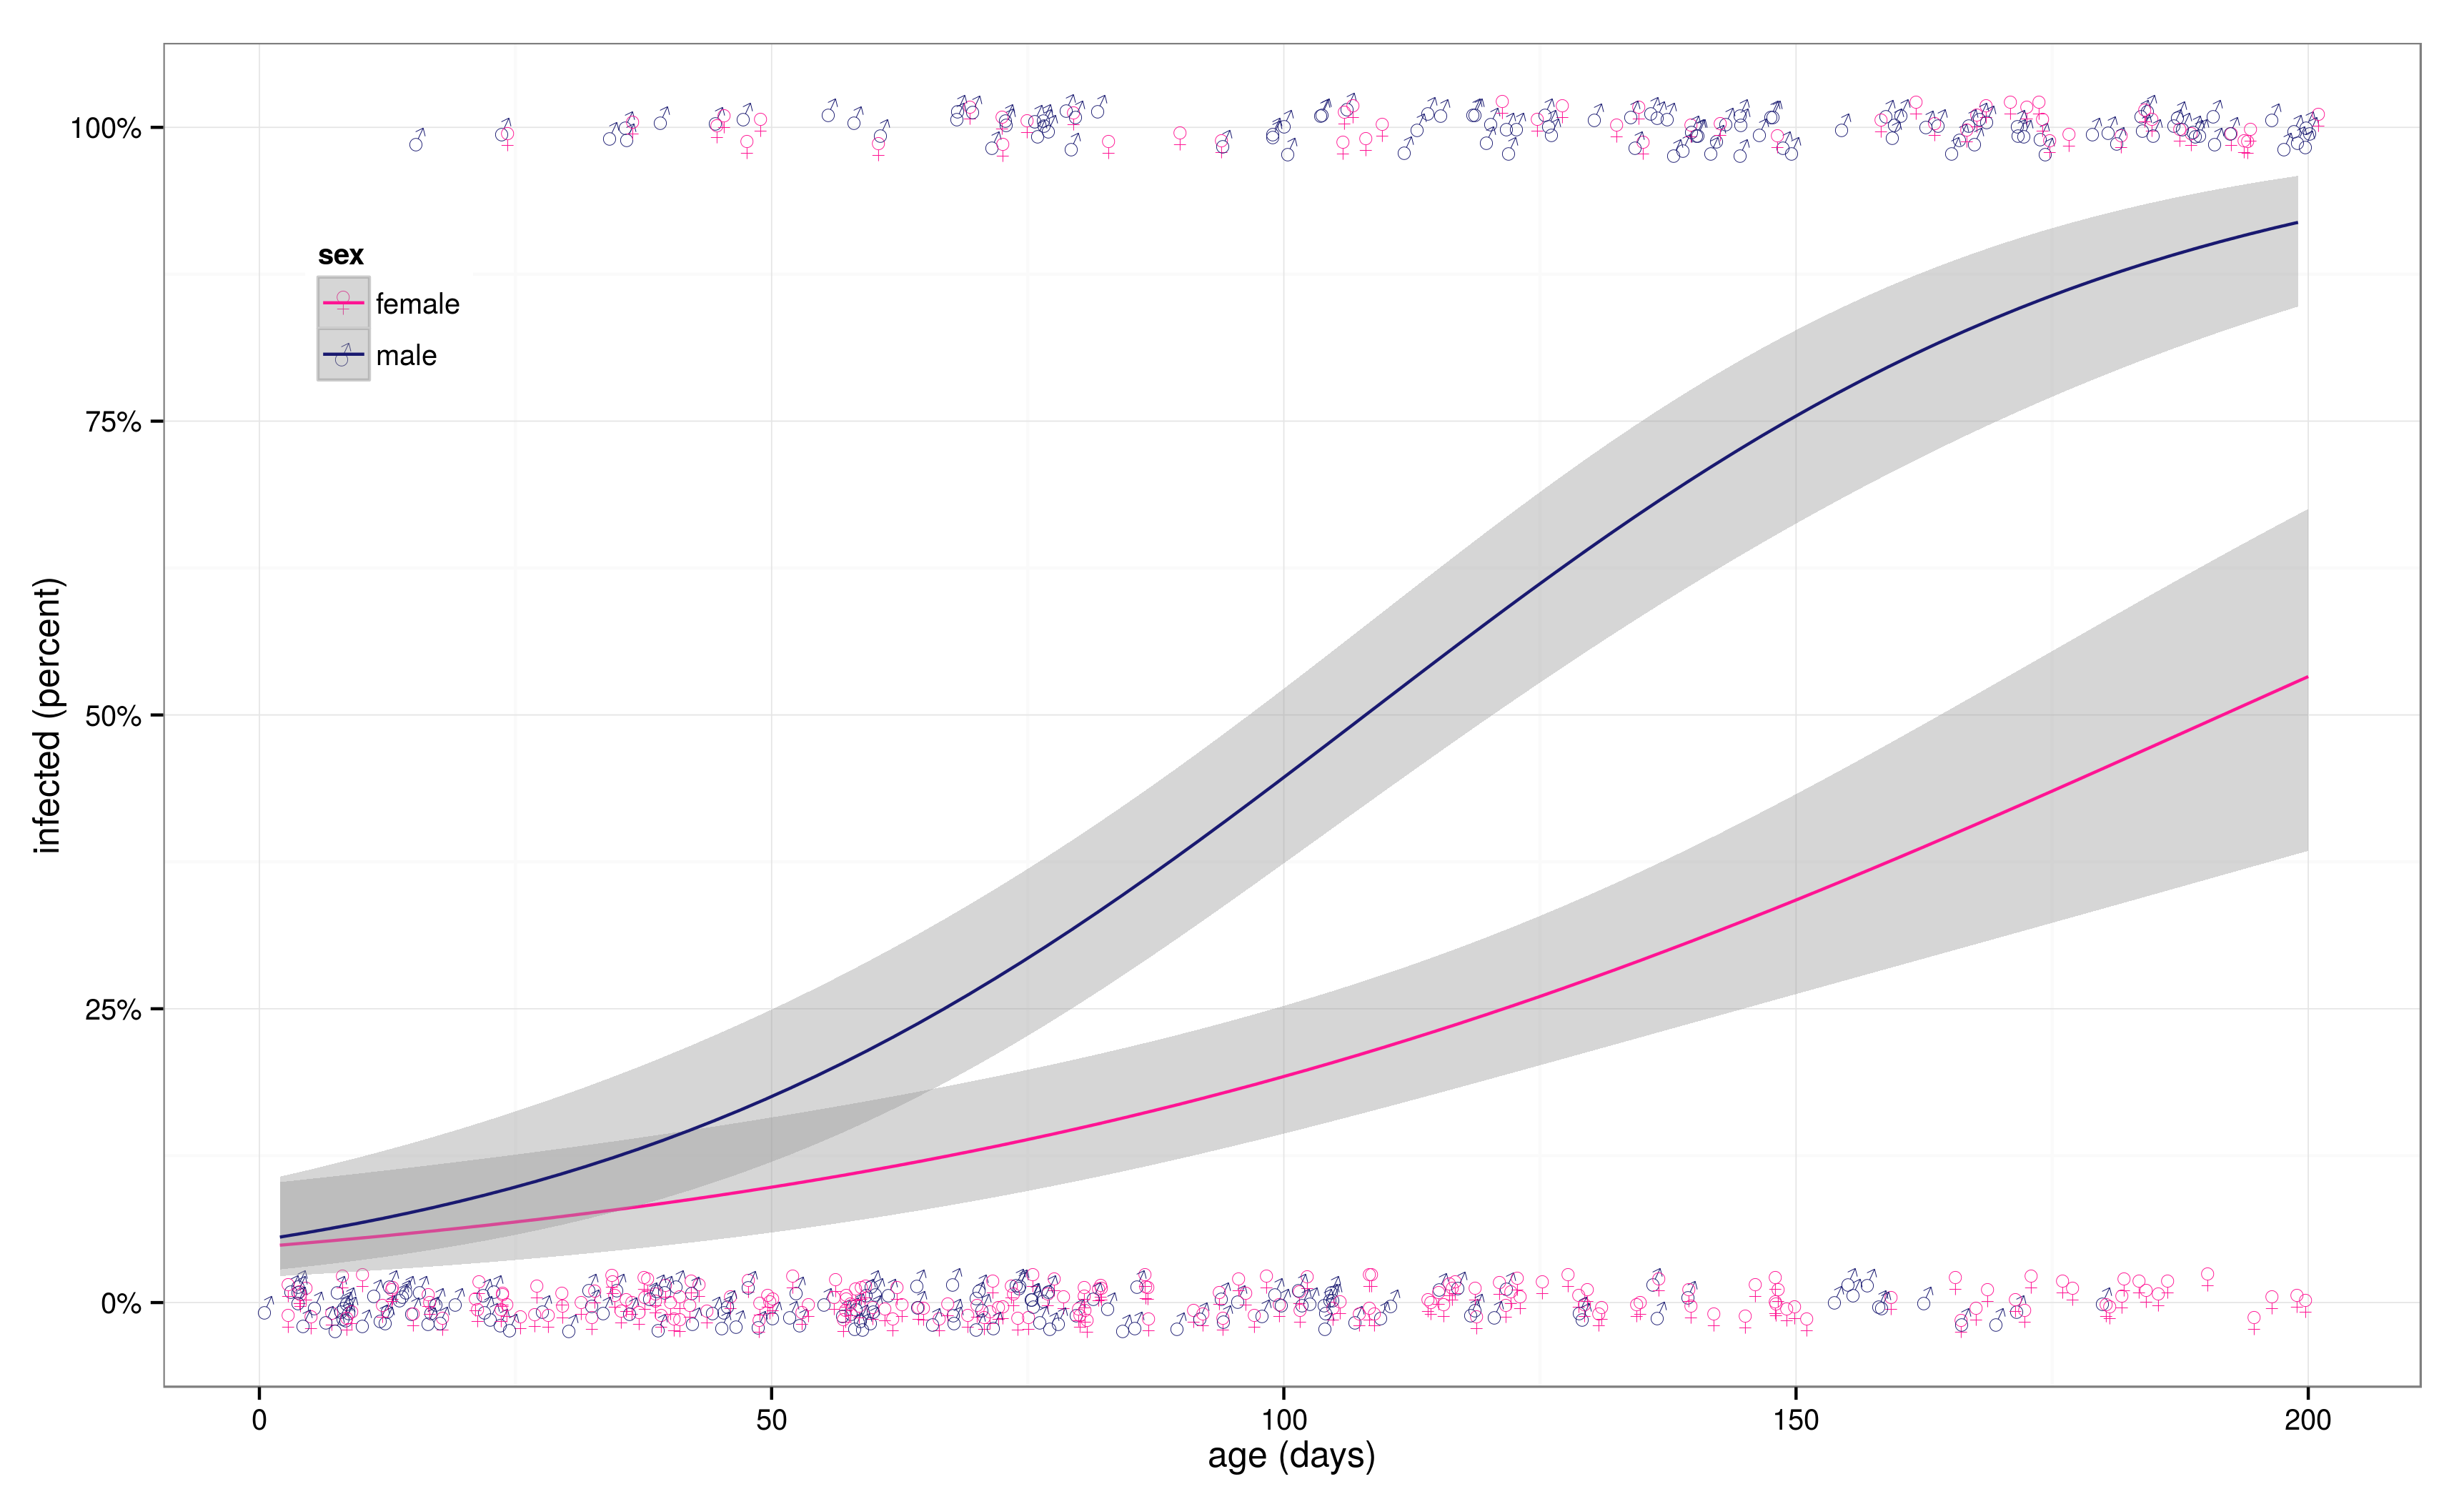
\includegraphics[width=11.5cm]{binancova1.png}
\end{center}
\end{frame}


\begin{frame}[fragile]\frametitle{Exercise}
Try to reproduce the plot! Hints:
  \begin{enumerate}
  \item set up a ggplot object, think about the aesthetics (\texttt{aes()}). Which quality of the graph you wanna set to which variable?
  \item begin with the lines (\texttt{geom\_smooth()})
  \item add the points (\texttt{geom\_jitter()}; do not think about the symbols in the first place; try to adjust the width and height appropriately)
  \item change the colour of the lines and points (\texttt{scale\_colour\_manual()}); I used midnightblue for male and deeppink for female
  \item change the symbols (\texttt{scale\_shape\_manual()}); use
\begin{verbatim}
    values = c("male" = "\u2642","female" = "\u2640"))
\end{verbatim}
     as values
  \item set the axes titles
  \item change to text of the y axis to percentage
  \item etc
  \end{enumerate}
\end{frame}


\begin{frame}[fragile]\frametitle{Exercise}
Try to reproduce the plot! Hints:
  \begin{enumerate}
  \item read the data melanoma.dat, you find a codebook under melanomacodebook.xlsx
  \item start by looking at the number of cases by each variable separately, ignoring age and sex (\texttt{table()})
  \item recode sex, skin complexion, hair colour, eye colour, freckles into factors; here is a example for sex
\begin{verbatim}
> mel$sex <- factor(mel$sex,labels=c("M","F"))
\end{verbatim}
  \item build up a model to see the effect of skin colour, look at hair eyes and freckles in the same way.
  \item now look at the effect of freckles, but control for age and sex
  \item try to find an appropriate way to visualize the last model
  \end{enumerate}
\end{frame}






\section{Multiple Numeric Regressors}
\begin{frame}\frametitle{Adjusting}
  \begin{itemize}
  \item what does it mean, this adjusting for the other variables?
  \item trying to describe a partial effect on an explanatory variable
  \item this information can be extracted from examination of the residuals
  \item so first: what are residuals?
  \end{itemize}
\end{frame}


\begin{frame}\frametitle{Residuals \& Errors}
  \begin{itemize}
  \item they are closely related but not the same
  \item error is the difference between an observed and a true value
  \item residual is the difference an observed value and an estimated (or fitted) value
  \end{itemize}
\end{frame}


\begin{frame}[fragile]\frametitle{Extracting Residuals}
  \begin{itemize}
  \item in R the function \texttt{resid()} is used to extract the residual from a fitted model
  \item as a example I use a data frame from the Scottish Hill Runners Association
    \begin{exampleblock}{Input/Output}\footnotesize
\begin{verbatim}
> m1 <- lm(time ~ climb + distance, data = sc.race)
> m1

Call:
lm(formula = time ~ climb + distance, data = sc.race)

Coefficients:
(Intercept)        climb     distance  
    -13.109       11.780        6.351  
\end{verbatim}
    \end{exampleblock}

  \end{itemize}
\end{frame}


\begin{frame}[fragile]\frametitle{Extracting Residuals}
  \begin{exampleblock}{Input/Output}\scriptsize
\begin{verbatim}
> resid(m1)
            1             2             3             4             5 
  5.654075838  -6.097514205  -1.949301243   1.652279007 -11.594100819 
            6             7             8             9            10 
  1.759046334  27.762266559   1.948712067   1.679667440   7.095732032 
           11            12            13            14            15 
  3.213520827   0.843507719  -8.141818080  13.242751997  -6.210948044 
           16            17            18            19            20 
-13.491402248  -3.301117259   6.052638082  -9.830881494   3.680216374
           21            22            23            24            25 
  6.471644737   1.110007329  -3.263474275   7.734520249   5.667604806 
           26            27            28            29            30 
 -9.635536908   0.008712067  -1.267352525   1.712107934  -3.586292630 
           31            32            33            34            35 
-16.653588589   0.314738687   7.784661945   2.616138471 -12.981222181 
\end{verbatim}
  \end{exampleblock}
\end{frame}


\begin{frame}[fragile]\frametitle{Residuals and Adjusting}
  \begin{itemize}
  \item suppose you have one outcome $y$ and two explanatory variables $x1$ and $x2$
  \item if you regress $y$ on a variable $x2$ (1)
  \item and $x1$ on $x2$ (2)
  \item and then the residuals from (1) on the residuals from (2)
  \item this last fit is identical to the partial effect of $x1$
  \end{itemize}
\end{frame}

\begin{frame}[fragile]\frametitle{Residuals and Adjusting}
  To get the partial effect of climb in model \texttt{m1}
  \begin{itemize}
  \item if you regress $time$ on a variable $climb$ (1)
    \begin{exampleblock}{Input}
\begin{verbatim}
> m.climb <- lm(time ~ distance, data = sc.race)
\end{verbatim}
    \end{exampleblock}
  \item and $climb$ on $distance2$ (2)
\begin{exampleblock}{Input}
\begin{verbatim}
> m.dist <- lm(climb ~ distance, data = sc.race)
\end{verbatim}
\end{exampleblock}
  \item and then the residuals from (1) on the residuals from (2)
\begin{exampleblock}{Input}
\begin{verbatim}
> m.res <- lm(resid(m.climb) ~ resid(m.dist))
\end{verbatim}
\end{exampleblock}
\end{itemize}
\end{frame}

\begin{frame}[fragile]\frametitle{Residuals and Adjusting}
\begin{exampleblock}{Input}\scriptsize
\begin{verbatim}
> m.res

Call:
lm(formula = resid(m.climb) ~ resid(m.dist))

Coefficients:
  (Intercept)  resid(m.dist)  
   -7.465e-16      1.178e+01  

> m1

Call:
lm(formula = time ~ climb + distance, data = sc.race)

Coefficients:
(Intercept)        climb     distance  
    -13.109       11.780        6.351  
\end{verbatim}
    \end{exampleblock}
\end{frame}



\begin{frame}\frametitle{Residuals and Adjusting}
  \begin{itemize}
  \item this concept also holds for partial correlation
  \item the \texttt{avPlots()} command (\texttt{car} package provides a feasible way to plot a partial effect
  \end{itemize}
\end{frame}


\begin{frame}[fragile]\frametitle{\texttt{avPlots()}}
\begin{verbatim}
> require(car)
> avPlots(m1)
\end{verbatim}
\begin{center}
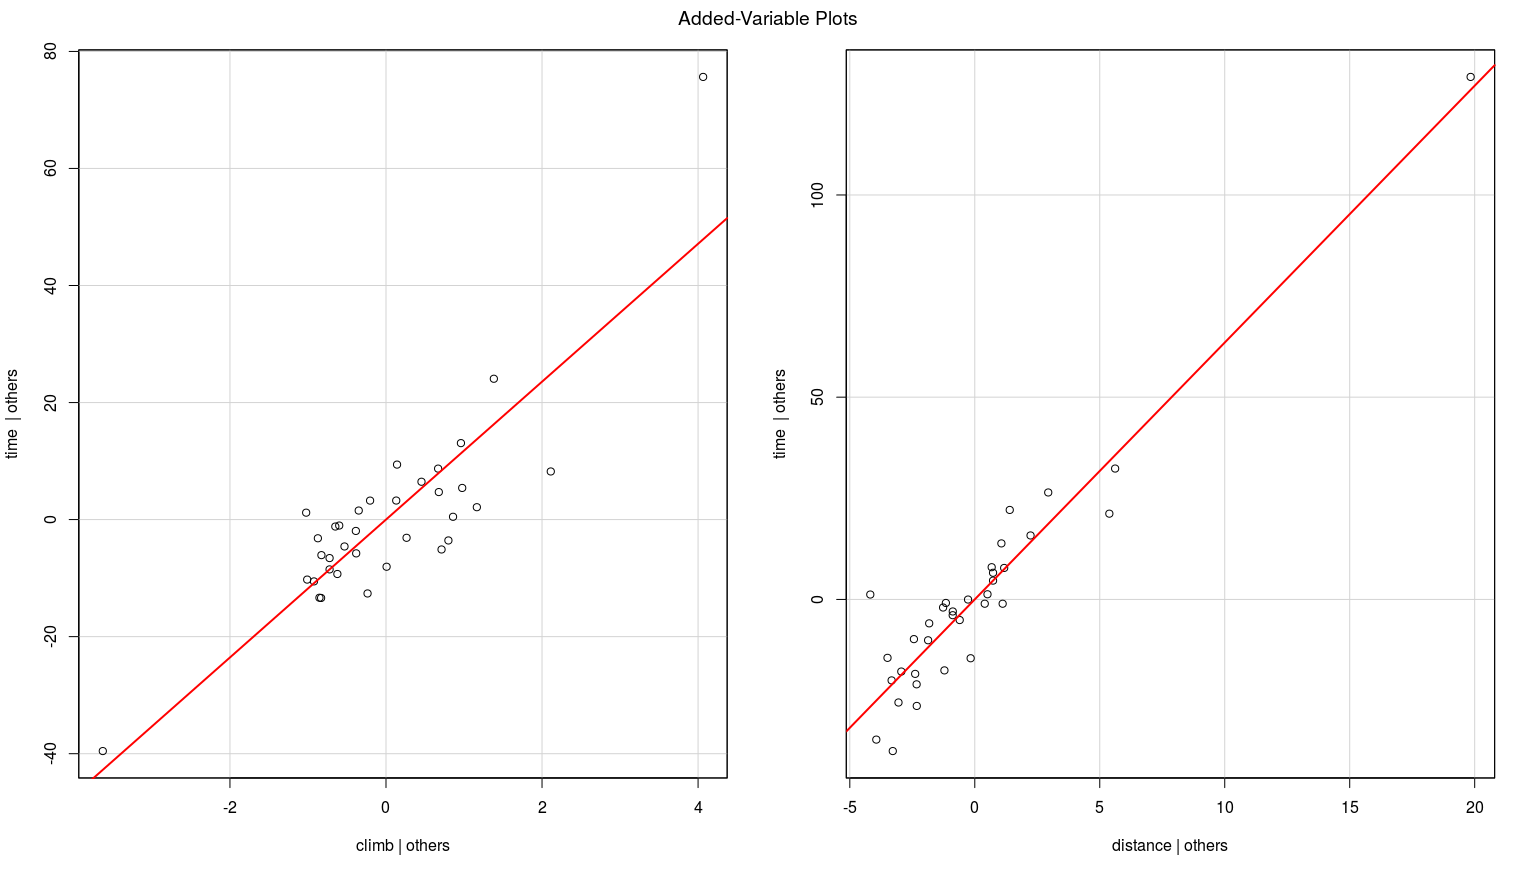
\includegraphics[width=11.5cm]{avplot1.png}
\end{center}
\end{frame}


\begin{frame}[fragile]\frametitle{\texttt{avPlots()}}
\begin{verbatim}
avPlot(m1,"climb")
\end{verbatim}
\begin{center}
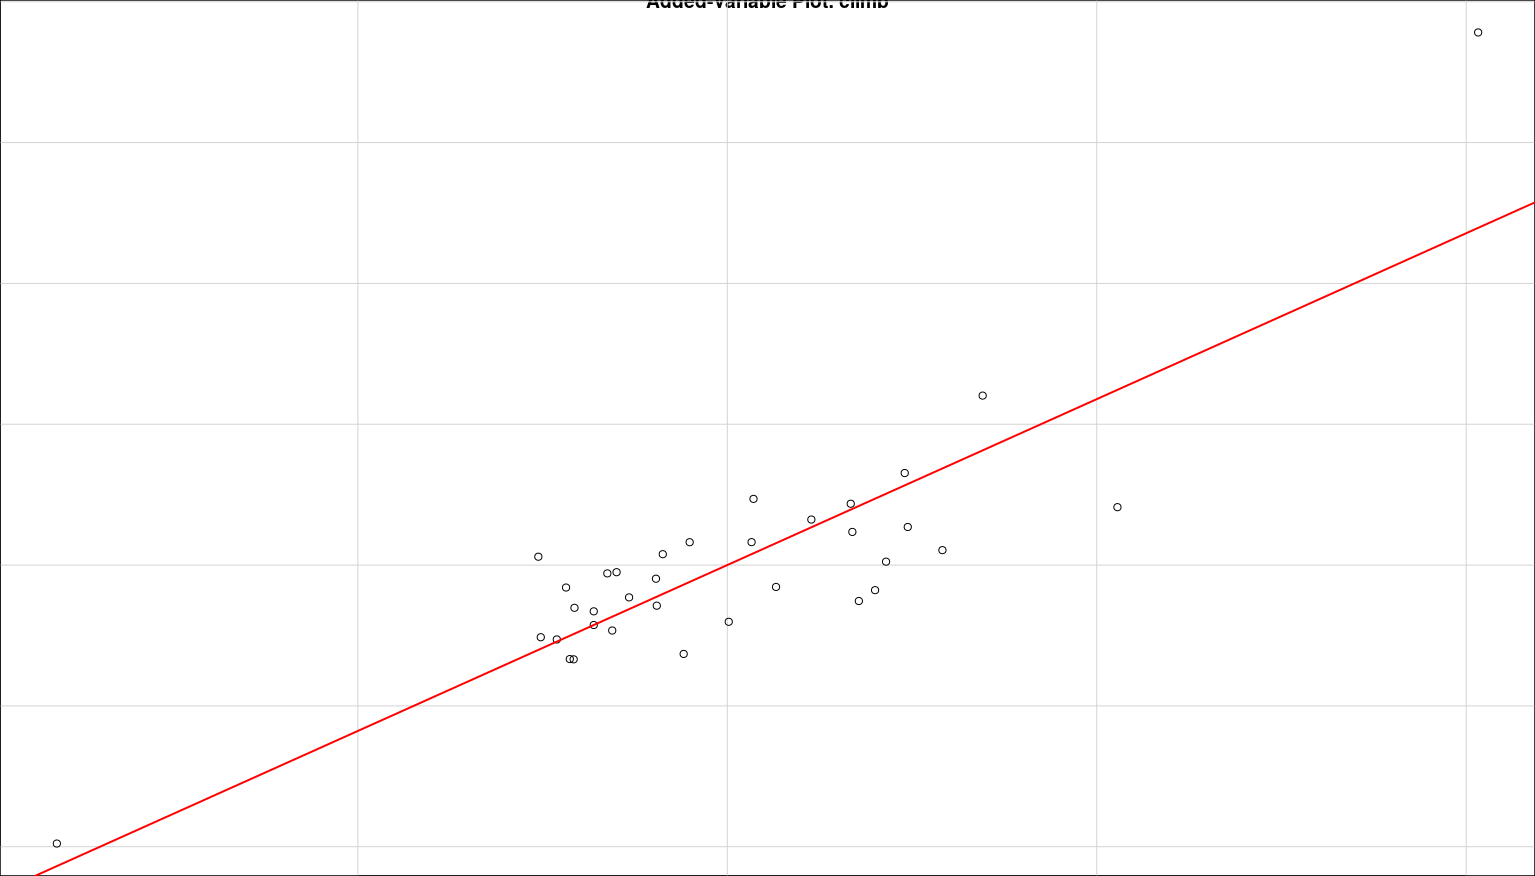
\includegraphics[width=10.5cm]{avplot2.png}
\end{center}
\end{frame}



\begin{frame}[fragile]\frametitle{\texttt{avPlots()}}
  \begin{itemize}
  \item avPlots also returns the aforementioned residuals
    \begin{exampleblock}{Input/Output}
\begin{verbatim}
> head(cbind(resid(m.dist),
+            avPlot(m1,"climb"),
+            resid(m.climb)))
                  climb       time           
1 -0.2037877 -0.2037877   3.253430   3.253430
2  0.9769679  0.9769679   5.411298   5.411298
3 -0.6230321 -0.6230321  -9.288702  -9.288702
4 -1.0098511 -1.0098511 -10.243901 -10.243901
5  1.1645426  1.1645426   2.124366   2.124366
6  0.9605426  0.9605426  13.074366  13.074366
\end{verbatim}
    \end{exampleblock}
  \end{itemize}
\end{frame}

\section{Summarizing the Fit of a Linear Model}
\begin{frame}\frametitle{Exercise}
  \begin{itemize}
  \item get the mean and the standard deviation of the three numeric variables in the \texttt{sc.race} data frame
  \item use the \texttt{pairs()} command and the \texttt{cor()} command to get a scatterplot matrix and the respective correlation matrix (Hint: these commands only work on numeric columns, so you have to get rid off the non-numeric ones. Remember indexing with negative integers)
  \end{itemize}
\end{frame}


\begin{frame}[fragile]\frametitle{Exercise}
  \begin{itemize}
  \item get the mean and the standard deviation of the three numeric variables in the \texttt{sc.race} data frame
  \end{itemize}
  \begin{exampleblock}{Input/Output}\tiny
\begin{verbatim}
> describe(sc.race[,-1])
         vars  n  mean    sd median trimmed   mad   min    max  range skew
distance    1 35  7.53  5.52   6.00    6.55  2.22  2.00  28.00  26.00 1.99
climb       2 35  1.82  1.62   1.00    1.54  0.74  0.30   7.50   7.20 1.68
time        3 35 56.09 50.39  36.37   46.46 20.95 15.95 204.62 188.67 1.77
         kurtosis   se
distance     3.83 0.93
climb        2.66 0.27
time         2.07 8.52
\end{verbatim}
  \end{exampleblock}
\end{frame}


\begin{frame}[fragile]\frametitle{Solution}
  \begin{itemize}
  \item get the correlation matrix
  \end{itemize}
  \begin{exampleblock}{Input/Output}\small
\begin{verbatim}
> M <- cor(sc.race[,-1])
> M
          distance     climb      time
distance 1.0000000 0.6523461 0.9430944
climb    0.6523461 1.0000000 0.8326535
time     0.9430944 0.8326535 1.0000000
\end{verbatim}
  \end{exampleblock}
\end{frame}


\begin{frame}[fragile]\frametitle{Solution}
  \begin{itemize}
  \item get the scatterplot matrix
  \end{itemize}
  \begin{exampleblock}{Input/Output}\small
\begin{verbatim}
> pairs(sc.race[,-1])
\end{verbatim}
  \end{exampleblock}
\end{frame}

\begin{frame}[fragile]\frametitle{Solution}
  \begin{itemize}
  \item get the scatterplot matrix
  \end{itemize}
\begin{center}
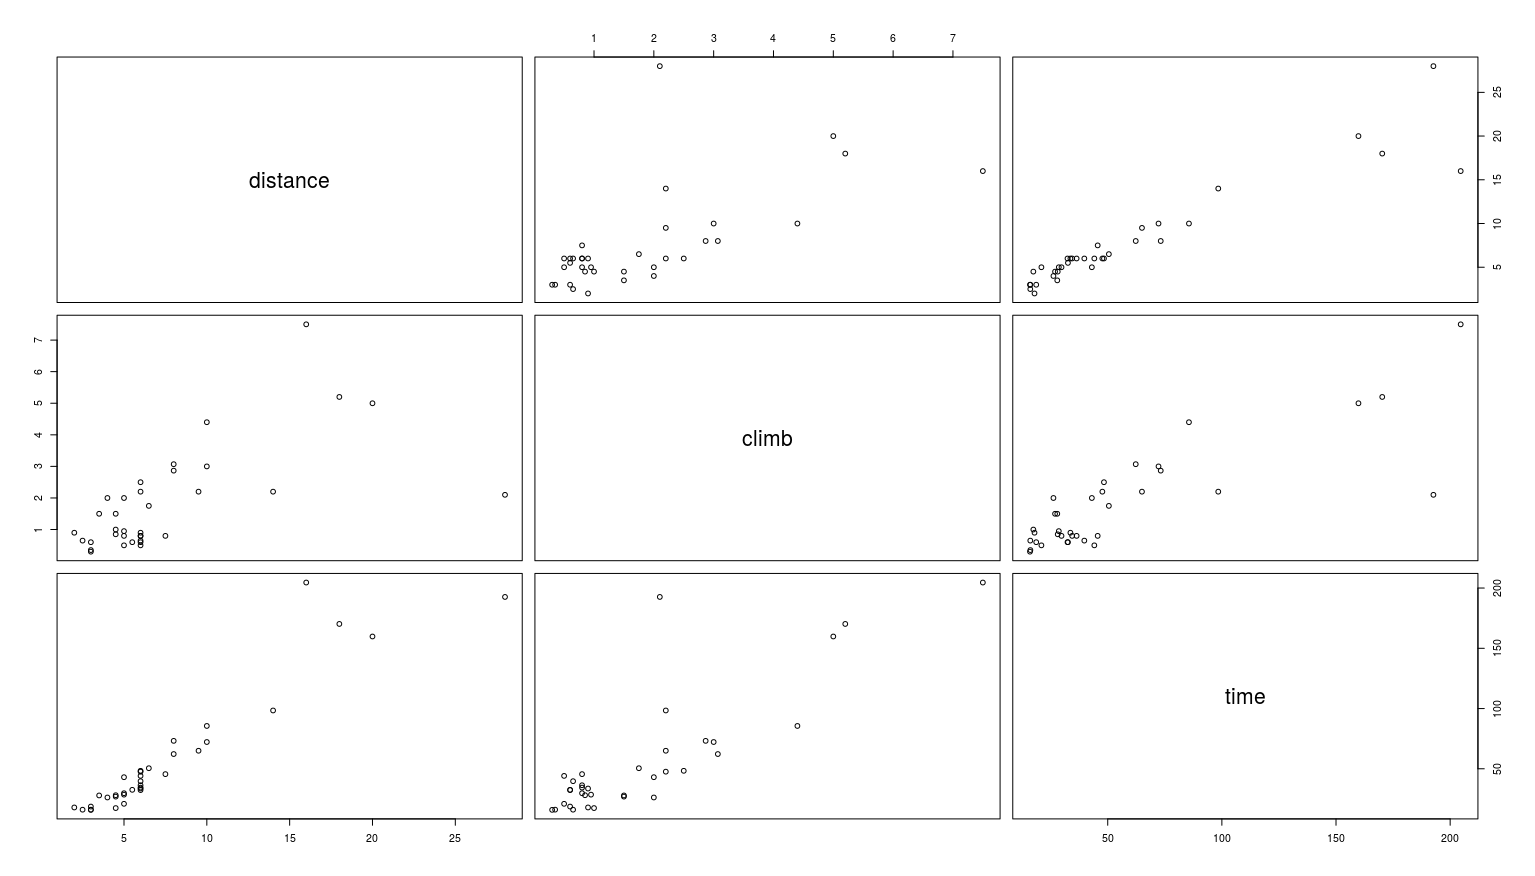
\includegraphics[width=11.5cm]{pairs1.png}
\end{center}
\end{frame}



\begin{frame}[fragile]\frametitle{Solution}
  \begin{itemize}
  \item get the scatterplot matrix
  \end{itemize}
  \begin{exampleblock}{Input/Output}\small
\begin{verbatim}
> pairs(sc.race[,-1],panel = panel.smooth)
\end{verbatim}
  \end{exampleblock}
\end{frame}

\begin{frame}[fragile]\frametitle{Solution}
  \begin{itemize}
  \item get the scatterplot matrix
  \end{itemize}
\begin{center}
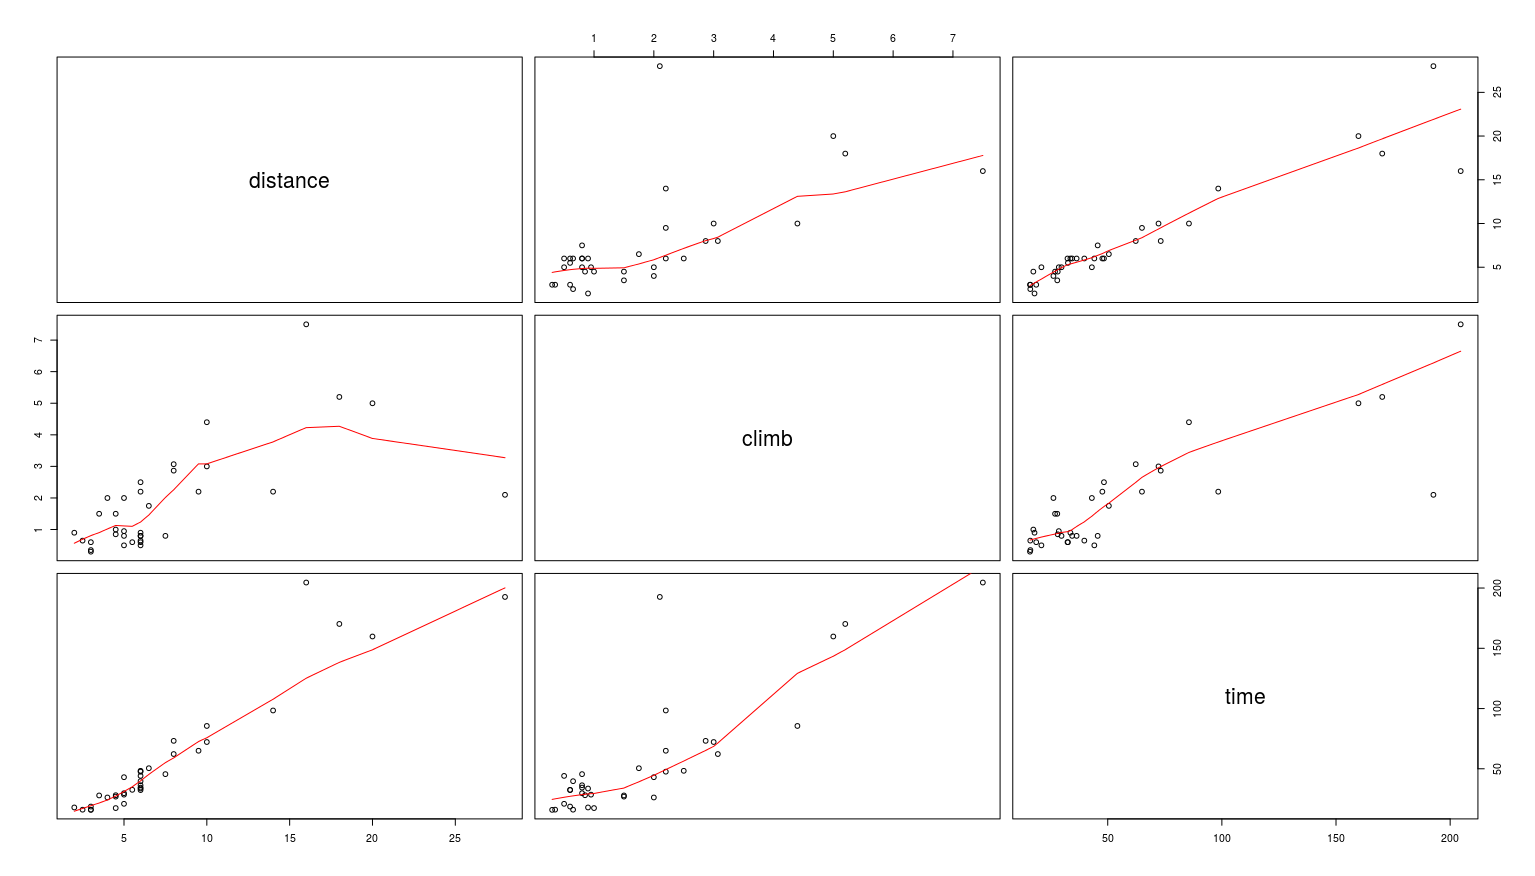
\includegraphics[width=11.5cm]{pairs2.png}
\end{center}
\end{frame}

